\documentclass[letterpaper]{article}  
\usepackage{graphicx}
\usepackage{float}
\usepackage[margin=0.5in]{geometry}
\usepackage{caption}
\usepackage{subcaption}
\usepackage{amsmath}
\usepackage{mathtools}

\usepackage{Sweave}
\begin{document}
\Sconcordance{concordance:hw4-sweave.tex:hw4-sweave.Rnw:%
1 9 1 1 0 143 1}


\title{STA511 Homework \#4}
\date{November 11, 2015}
\author{Abbas Rizvi}
\maketitle

\begin{enumerate}
\item 
\begin{enumerate}
\item The log likelihood function of the poisson pdf, $f(x) = \frac{\lambda^{x}e^{-\lambda}}{x!}$ was derived to be $log(\lambda) = \sum X_{i} log(\lambda) \cdot -n\lambda$. The log likelihood function of the given observations are plotted in Figure 1. 

The code can be seen below:

\begin{verbatim}
counts <- c(rep(0,7840), rep(1,1327), rep(2,239), rep(3,42), rep(4,14), rep(5,4), rep(6,4), rep(7,1))

n <- length(counts)

neglikefun <- function(lambda){
        n*lambda-sum(counts)*(log(lambda))
}

lambda <- seq(0.00001, 1, length=1000)

library(ggplot2)
qplot(lambda, 
      sapply(lambda, function(lambda){-1*neglikefun(lambda)}),
      geom = 'line',
      main = paste('Log Likelihood as a Function of', sep=" ", expression(lambda)),
      xlab = expression(lambda),
      ylab = 'Log Likelihood')
\end{verbatim}
\begin{figure}
\centering
\caption{Question 1}
\centering
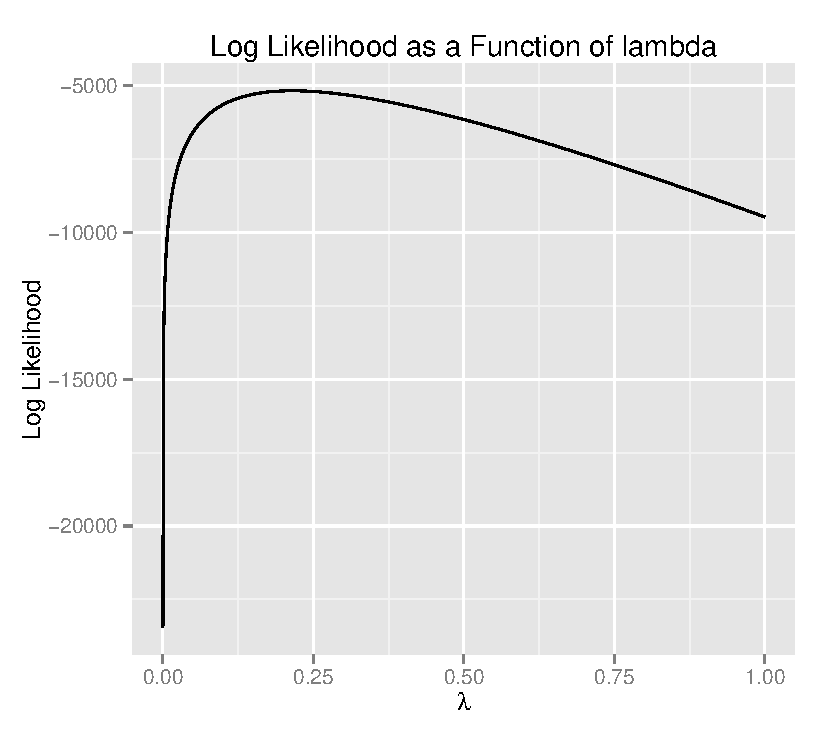
\includegraphics{/Users/aarizvi/Desktop/ROSWELL_PHD/STA511_StatisticalComputing/HW4/hw4-q1a.pdf}
\end{figure}
\item The MLE of $\lambda$ was computed as 0.2151832. The R code that was used to compute this answer can be seen below:

\begin{verbatim}
nlminb(1,function(lambda){neglikefun(lambda)})
$par
[1] 0.2151832
\end{verbatim}

\item The probability that a randomly selected policy has 2 claims (g($\lambda$)) = Pr($Y_{i} = 2$)) was estimated to be 0.1866955. This was computed by simply plugging in $\lambda_{MLE}$ into the Poisson pdf. The R code that was used to compute this answer can be seen below:
\begin{verbatim}
> ((0.2151832^2)*(exp(-0.2151832)))/factorial(2)
[1] 0.01866955
\end{verbatim}
\end{enumerate}
\item
\begin{enumerate}
\item $\theta_{MLE}$ was computed by taking the log likelihood of the normal distribution pdf, $f(x) = \frac{1}{\sigma\sqrt{2\pi}}e^{-(x-\mu)^{2}/2\sigma^{2}}$. The calculations for finding $\theta_{MLE}$ can be seen below: 

$$ L(\theta) = \prod\limits_{i=1}^{n} \frac{1}{\sqrt{2\pi}} e^{-(x - \theta)^{2}/2} $$

$$ \ell(\theta) = -\frac{n}{2} log(2\pi) - \frac{\sum\limits_{i=1}^{n} (X_{i} - \theta)^{2}} {2} $$

$$ \ell'(\theta) = \sum\limits^{n}_{i=1} X_{i} - n\theta = 0 $$

$$ \hat{\theta}_{MLE} = \frac{\sum\limits^{n}_{i=1} X_{i}}{n} = \bar{X} $$ 

\item The question prompt said $\Phi = Pr(Y_{i} = 1)$ -- and according the given piecewise function of $Y_{i}$, $Y_{i} = 1$ is true only when $X_{i} > 0$. Computing the cdf of a normal distribution is not trivial using integration. As such, using the rules of probability we can represent the normal distribution function as a cdf. $\Phi_{MLE} = g(\hat{\theta}_{MLE})$ where $g(\theta)= 1 - F(0)$. Where F(x) is the cdf of a standard normal distribution N(0,1). 


$$ P (X \leq 0) = P \Bigg( \frac{X - \theta}{1} \leq \frac{0 - \theta}{1} \Bigg) $$

And because $F(x) = g(\frac{x-\mu}{\sigma}) = g(Z)$ when $X \sim N(0,1)$

$$= P (Z \leq {-\theta})$$

Therefore,

$$ \Phi_{MLE} = 1 - F(-\hat{{\theta}}) $$

\item We were asked to compute the asymptotic standard error for $\theta$ and for $\Phi$. 

In order to compute $se(\theta)$, the theorem that of asymptotic normality was utilized, that states that the standard error is the square root of 1 / Fisher Information $(se = \frac{1}{\sqrt{I_{n}(\theta)}}).$


$$ \hat{se}(\hat{\theta}_{MLE}) = \sqrt{\frac{1}{I_{n}(\hat{\theta}_{MLE})}} $$
$$ I_{n}(\theta) = -nE \Bigg[ \frac{\delta^{2}}{\delta\theta^{2}} log f(x\vert\theta) \Bigg] = -nE \Bigg[ \frac{\delta^{2}}{\delta\theta^{2}} {-\frac{1}{2}} log (2\pi) - \frac{(x-\theta)^{2}}{2}\Bigg] = -nE \Bigg[ \frac{\delta}{\delta(\theta)} (x-\theta) \Bigg] = -nE \big[-1\big] = n $$
$$\hat{se}(\hat{\theta}_{MLE}) = \sqrt{\frac{1}{n}} $$

We can use the Delta Method to compute $\hat{se}(\hat{\Phi}_{MLE})$. 

$$\hat{se}(\hat{\Phi}_{MLE}) = \big|g'(\hat{\theta}_{MLE})\big| \cdot \hat{se}(\hat{\theta}_{MLE}) $$
$$ g'(\theta) = {-{\frac{1}{1}}} \frac{1}{\sqrt{2\pi}} e^{-(\theta-\mu)^{2} / 2 \cdot 1} $$

Standard $X_{i} \sim N(0,1)$ was assumed for $g'(\theta)$, so 0 were plugged in for $\mu$ and 1 was plugged in for $\sigma^{2}$.

$$ = \Bigg| \frac{1}{\sqrt{2\pi}}e^{-(\theta)^{2}/2} \Bigg| $$

And finally, 

$$ \hat{se}(\hat{\theta}_{MLE}) = \Bigg|\frac{1}{\sqrt{2\pi}}e^{-\bar{X}^{2}/2}\Bigg| \cdot \sqrt{\frac{1}{n}} $$


\end{enumerate}
\item
\begin{enumerate}
\item 
Since the likelihood is the joint distribution of the data which is equivalent to the product of marginal distributions, we can multiply the marginal distributions: 
$$ L(\theta) = \prod\limits_{i=1}^{n} \frac{1}{\theta} e^{-{X_{i}/\theta}} \cdot \prod\limits_{i=1}^{m}e^{-5Y_{i}/\theta}\cdot (1 - e^{5/\theta})^{1-Y_{i}} $$

$$ L(\theta) = \frac{1}{\theta^{n}}e^{-\sum\limits^{n}_{i=1}X_{i}/\theta} \cdot e^{\sum\limits^{m}_{i=1}-5Y_{i}/\theta} \cdot \big(1 - e^{-5/\theta}\big)^{\sum\limits^{m}_{i=1}(1-Y_{i})} $$

\item 
To MLE for $\theta$ was calculated to be 5.971734. The MLE was computed by taking the logarithm of the likelihood function as follows:

From part 3(a):
$$l(\theta) = -nlog(\theta) - \sum^{n}_{i=1}{\frac{X_{i}}{\theta}} + \sum^{m}_{i=1}{\frac{5Y_{i}}{\theta}} + \sum^{m}_{i=1}{(1-Y_{i})log(1-e^{-5/\theta})}$$

%$$l'(\theta) = \frac{-n}{\hat{\theta}} + \frac{\sum{X_{i}}}{\hat{\theta^{2}}} + \sum^{m}_{i=1}\frac{5Y_{i}}{\theta^{2}} + \sum^{m}_{i=1}{m - Y_{i}} \cdot \frac{1}{1-e^{-5/\theta}} \cdot e^{5} \cdot \frac{5}{\theta^{2}}$$

$\theta_{MLE}$ was then calculated by taking this log likelihood function and using the optimize function in R. The code can be seen below:

\begin{verbatim}
> f.obs <- c(2.8, 5.6, 24.7, 6.5, 1.6, 10.6, 1.0, 7.8, 7.2, 13.9)
> n <- length(f.obs)
> g.obs <- c(0,0,0,1,1,1,0,0,1,0,0,0,0,0,0)
> m <- length(g.obs)
> 
> likefun <- function(theta){
+         -n*log(theta)-sum(f.obs)/theta-5*sum(g.obs)/theta+(m-sum(g.obs))*log(1-exp(-5/theta))
+ } 
> 
> optimize(likefun, c(10,0), maximum=TRUE)
$maximum
[1] 5.971734

$objective
[1] -41.13977

\end{verbatim}

\end{enumerate}
\end{enumerate}

\end{document}
